\documentclass[a4paper,12pt]{article}
\usepackage{amsmath}
\usepackage{cite}
\usepackage{graphicx}
\usepackage{amssymb}
\graphicspath{ {diagram/} }



\begin{document}
\title{Remarks}
\author{Linh Dang}
\date{05.03.15} 
\maketitle

\section*{Protein-Protein Interface for Homologous Protein Complexes}
\subsection*{Situation}
Homologous protein is a complex where there are two identical protein chain sequences (could be different 3D structure). Though it is the simple complex, it comprises several difficulties when dealing with Direct Coupling Method:
\begin{enumerate}
\item
If two MSAs derived from these two chains are completely identical, the DCA algorithm could not distinguish the score of pair intra-protein or inter-protein (as in below figure). And because the big MSA contains a lot of identical pair of column, it will throws error in computation.
\item
All the scores of inter-consecutive pair (A($ S_1 $)-B($ S_2 $); A($ S_2 $)-B($ S_3 $); and so on) are relatively large and therefore it does not make sense.
\item
The average length of protein sequence is about 350, which means the concatenated one is 700. Thus, the matrix contains all information of pair of amino acids is around 14000 x 14000. And in some case, it takes more than ten hours to compute one protein complex, and most of the time using for the matrix inversion. This issue could be overcome by using GPU. However, if a protein sequence is longer than 500, it demands a huge memory to temporarily save the matrix, which could easily trigger the out of memory exception. 

\end{enumerate}
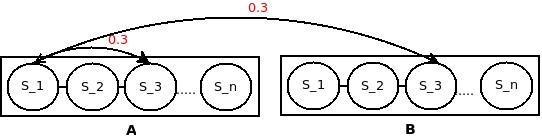
\includegraphics[width=\textwidth]{HomologousProteinComplex.jpeg}

\subsection*{Resolution}
There are so far at least two perpendicular ways to enhance the situation. Firstly, we could improve the concatenated MSA of complex based on the following observation. Though two chains in complex are identical, their descendants/ancestors in the evolutionary process could have a bit differences. Secondly, we could utilize other version of approximations to improve the Ising model in order to tailor it to our problem. 
\subsubsection*{New approach to create concatenated MSA}

Two MSAs could be not completely identical even if their query sequences are the same. Using the method described in \cite{Hopf2014}, we can construct concatenated MSA for two protein chains in complex. In short, two sequences in concatenated MSA are put together if and only if their corresponding proteins are close proximity in genome (or on the same operon). Thus, the two corresponding proteins satisfy two conditions

\begin{enumerate}
\item
CDS of each concatenated protein pair must be located on the same genomic contig.
\item
Each pair must be the closest to one another on the genome.
\end{enumerate}

\subsubsection*{Improve Ising model}

In general, the Hamiltonian of Ising model is defined by
\begin{equation} \label{eq1}
 -\mathbf{H}_{A,\textbf{h}}(\sigma) \stackrel{def}{=}  \sum_{i,j \in \Lambda} \mathbf{J}_{ij}\sigma_i \sigma_j + \sum_{i \in \Lambda} h_i \sigma_i 
\end{equation}
The probability of the configuration of spin is
\begin{equation} \label{eq2}
 \mathbf{P}_{\mathbf{J},\textbf{h}}(\sigma) \stackrel{def}{=}  \frac{1}{Z}exp(-\mathbf{H}) 
\end{equation}
where $ Z $ is partition function, or the normalizing factor.
And the average magnet per site at position $ \textbf{i} $ is
\begin{equation} \label{eq3}
<m_\textbf{i}> = \sum_\sigma{\frac{1}{Z}\sigma_\textbf{i}exp(-\mathbf{H})}
\end{equation}
And the correlation between two sites $ i,j $ is
\begin{equation}\label{eq4}
 \mathbf{C}_{ij}=<m_im_j> - <m_i><m_j>
\end{equation}
However, $ <m_\textbf{i}> $ could be calculate directly through MSA in order to make it consistent with the data.

The direct Ising model problem is that given the configuration $ \mathbf{J}_{ij} $ and external magnetic field $ h_i $, the problem is how to calculate the free energy $ -log(Z) $ and the average value of magnet.

However, we are only  interested in the inverse Ising model which is defined as following. Given the M configurations of the spin (corresponding to M lines in MSA), we'd like to estimate the coupling and fields ($ \mathbf{J}, h $).
\subsubsection{Naive Mean Field Approximation (nMF)}
In \cite[Morcos11], the authors use naive mean field approximation, which based on two main assumptions \cite[Chap5Ising]: (i) neglects spin fluctuations around the mean, and (ii) considers spins to behave statistically independently. Then the result is
\begin{equation}\label{eq5}
\mathbf{J}_{ij}^{nMF} = -(\mathbf{C}^{-1})_{ij}
\end{equation}

Other a bit advanced approximations are following.
\subsubsection{nMF with Onsager reaction term (TAP)}
\begin{equation}\label{eq6}
\mathbf{J}_{ij}^{TAP} = \frac{\sqrt{1-8m_im_j(\mathbf{C}^{-1})_{ij}}-1}{4m_im_j}
\end{equation}
\subsubsection{Bethe Approximation (BA)}
\begin{multline} 
\mathbf{J}_{ij}^{BA} = -atanh \Bigl[ \frac{1}{2(\mathbf{C}^{-1})_{ij}}\sqrt{1+4(1-m_i^2)(1-m_j^2)((\mathbf{C}^{-1})_{ij}^2)} -m_im_j \\
-\frac{1}{2(\mathbf{C}^{-1})_{ij}}\sqrt{{\left( \sqrt{1+4(1-m_i^2)(1-m_j^2)((\mathbf{C}^{-1})_{ij}^2)}-2m_im_j\mathbf{C}^{-1})_{ij} \right)}^2 -4(\mathbf{C}^{-1})_{ij}^2} \Bigr]
\end{multline}

\subsubsection*{Pseudo-Maximum LogLikelihood}
Given a set of M configurations, instead of calculate the loglikelihood of $\amalg_{b=1}^M P(\sigma^{(b)})$, which is
\begin{equation}\label{eq7}
l=\sum_{b=1}^M \log \mathbf{P} \left( \sigma^{(b)} \right)
\end{equation}

we calculate the conditional probability of observing one variable $ \sigma_r $ given observations of all the other variables $ \sigma_{\setminus r} $. Thus, we have
\begin{equation}\label{eq8}
\mathbf{P} \left( \sigma_r=\sigma^{(b)} | \sigma_{\setminus r}^{(b)} \right) = \frac{\exp [\sigma_i(h_i+ \sum_j \mathbf{J}_{ij}s_j)]}{2cosh \left( h_i+\sum_j \mathbf{J}_{ij}s_j \right)}
\end{equation}

Consequently, the pseudo log likelihood is
\begin{equation}\label{eq9}
l_{pseudo} = \sum_{r=1}^N \sum_{b=1}^M \log \left[ \mathbf{P}_{h_r,J_r} \left( \sigma_r=\sigma^{(b)} | \sigma_{\setminus r}=\sigma_{\setminus r}^{(b)} \right) \right]
\end{equation}


\begin{thebibliography}{1}

  \bibitem{Hopf2014} Thomas A Hopf et. al. Sequence co-evolution gives 3D contacts and structures of protein complexes. Elife.
\bibitem{Morcos11} Morcos, F., Pagnani, A., Lunt, B., Bertolino, A., Marks, D.S., Sander, C., Zecchina, R., Onuchic, J.N., Hwa, T., Weigt, M. Direct-coupling analysis of residue coevolution captures native contacts across many protein families. Proc Natl Acad Sci USA 108, E1293-E1301 (2011).
\bibitem{Federico} Federico Ricci-Tersenghi. A brief introduction to the inverse Ising problem and some algorithms to solve it.
\bibitem{Chap5Ising}. Mean Field Treaments  of the Ising Model. Chapter 5: Mean-Field Theory. Unknown authors.

  \end{thebibliography}
\end{document}